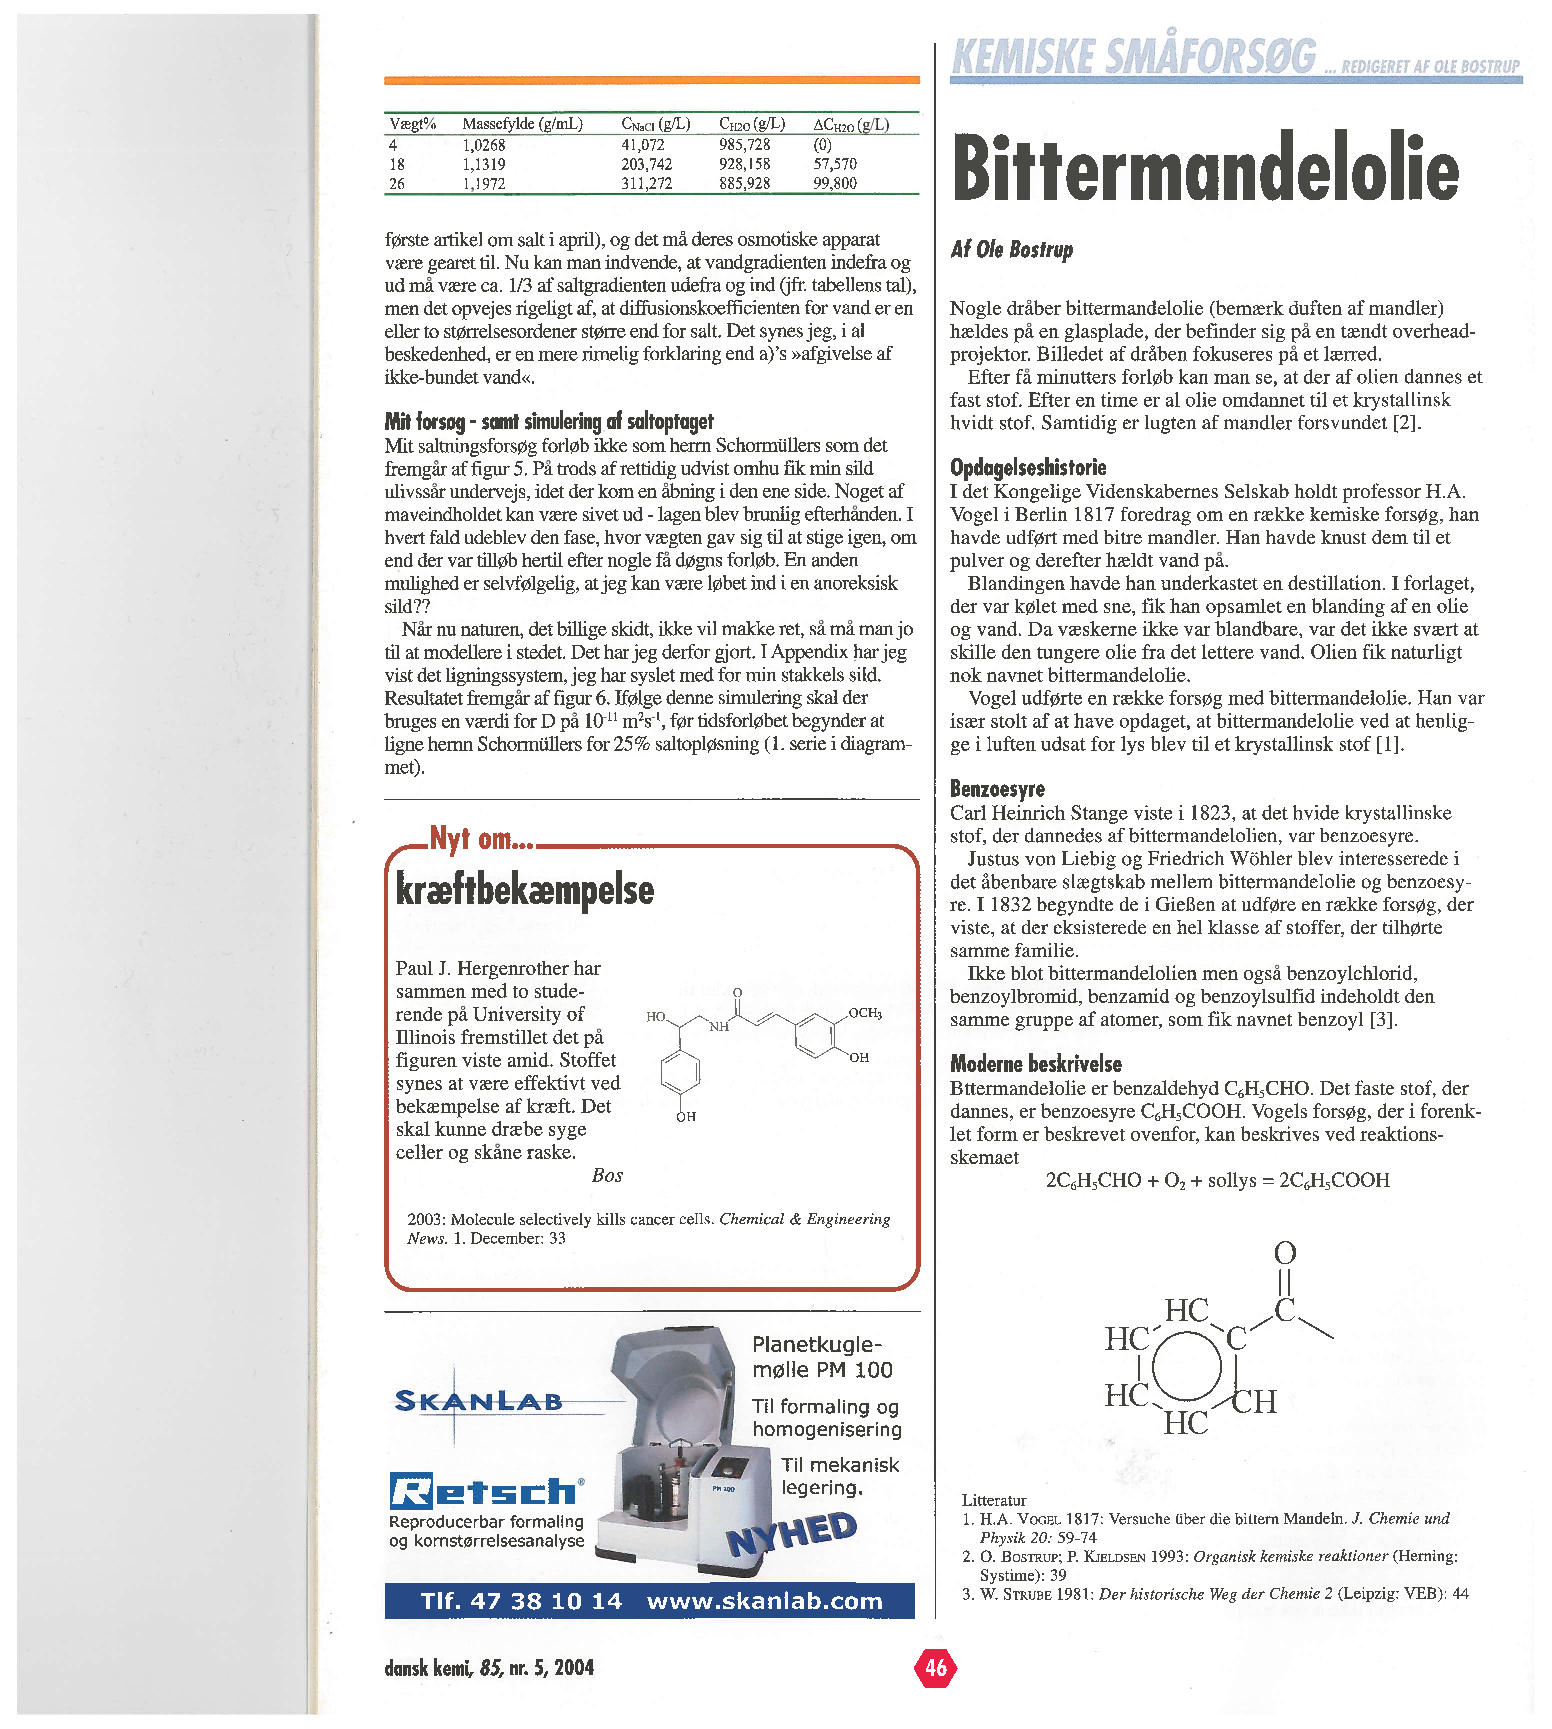
\includepdf[pages=-]{pdfs/2004-85-5-46.pdf}
\emne{Bittermandelolie}


\danskkemi{85 nr. 5, s. 46}

Nogle dråber bittermandelolie (bemærk duften af mandler) hældes på en glasplade, der befinder sig på en tændt overheadprojektor. Billedet af dråben fokuseres på et lærred.
Efter få minutters forløb kan man se, at der af olien dannes et fast stof. Efter en time er al olie omdannet til et krystallinsk hvidt stof. Samtidig er lugten af mandler forsvundet [2].

\deloverskrift{Opdagelseshistorie}

I det Kongelige Videnskabernes Selskab holdt professor H.A. Vogel i Berlin 1817 foredrag om en række kemiske forsøg, han havde udført med bitre mandler. Han havde knust dem til et pulver og derefter hældt vand på.
Blandingen havde han underkastet en destillation. I forlaget, der var kølet med sne, fik han opsamlet en blanding af en olie og vand. Da væskerne ikke var blandbare, var det ikkesvært at skille den tungere olie fra det lettere vand. Olien fik naturligt nok navnet bittermandelolie.
Vogel udførte en række forsøg med bittermandelolie. Han var især stolt af at have opdaget, at bittermandelolie ved at henligge i luften udsat for lys blev til et krystallinsk stof [1].

\deloverskrift{Benzoesyre}
Carl Heinrich Stange viste i 1823, at det hvide krystallinske stof, der dannedes af bittermandelolien, var benzoesyre.
Justus von Liebig og Friedrich Wöhler blev interesserede i det åbenbare slægtskab mellem bittermandelolie og benzoesyre. I 1832 begyndte de i Gießen at udføre en række forsøg, der viste, at der eksisterede en hel klasse af stoffer, der tilhørte samme familie.
Ikke blot bittermandelolien men også benzoylchlorid, benzoylbromid, benzamid og benzoylsulfid indeholdt den samme gruppe af atomer, som fik navnet benzoyl [3].

\deloverskrift{Moderne beskrivelse}
Bittermandelolie er benzaldehyd \ch{C6H5CHO}. Det faste stof, der dannes, er benzoesyre \ch{C6H5COOH}. Vogels forsøg, der i forenklet form er beskrevet ovenfor, kan beskrives ved reaktionsskemaet

\ch{2 C6H5CHO + O2 + sollys = 2 C6H5COOH}

\chemfig{
                   O% 8
            =[:270]% 7
                      (
                -[:330]% 9
                      )
            -[:210]% 3
            -[:270]% 2
            -[:210]% 1
                      (
    -[:90,,,,draw=none]\mcfcringle{1.3}% (o)
                      )
            -[:150]% 6
             -[:90]% 5
             -[:30]% 4
                      (
                -[:330]% -> 3
                      )
}

Litteratur
H.A. Vogel, 1817: Versuche über die bittern Mandeln. J.Chemie und Physik 20: 59-74
O.Bostrup, P.Kjeldsen 1993, Organisk kemiske reaktioner (Herning: Systime): 39
W. Strube 1981: Der historische Weg der Chemie 2 (Leipzib: VEB):44
